%%%%%%%%%%%%%%%%%%%%%%%%%%%%%%%%%
%
%       EXERCÍCIO
%
%%%%%%%%%%%%%%%%%%%%%%%%%%%%%%%%%

\ifdefstring{\atividade}{prova}{%
    \ifdefstring{\modo}{objetivo}{%
        \renewcommand{\valorquestao}{\ValorQObj\ ponto}
    }{%
        \renewcommand{\valorquestao}{\ValorQDisc\ pontos}
    }%
}%

\begin{exercicioBanco}[\valorquestao]
Das figuras a seguir, indique aquela que representa o gráfico de uma função real \(f:[a,b] \to \mathbb{R}\), onde \(a,b \in\mathbb{R}\).

% Define as alternativas
\newcommand{\alternativas}{%
    \begin{center}
        \begin{tabularx}{\textwidth}{XXX}
            \hspace{40pt} (a) & \hspace{40pt} (b) & \hspace{40pt} (c) \\[6pt]

            %----------------- A -----------------
            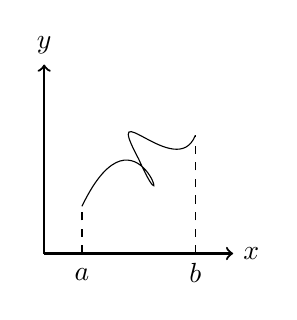
\begin{tikzpicture}[scale=0.6]
            \draw[->,thick] (0,0)--(4,0) node[right]{$x$};
            \draw[->,thick] (0,0)--(0,4) node[above]{$y$};
            \draw[dashed] (0.8,0)--(0.8,1);
            \draw[dashed] (3.2,0)--(3.2,2.5);

            % Curva com laço
            \draw (0.8,1)
                  .. controls (2,3.5) and (2.8,0.2) ..
                  (2,2)
                  .. controls (1.2,3.5) and (2.8,1.5) ..
                  (3.2,2.5);

            \node[below, yshift=-2pt] at (0.8,0) {$a$};
            \node[below] at (3.2,0) {$b$};
            \end{tikzpicture}

            %----------------- B -----------------
            &
            \begin{tikzpicture}[scale=0.6]
            \draw[->,thick] (0,0)--(4,0) node[right]{$x$};
            \draw[->,thick] (0,0)--(0,4) node[above]{$y$};
            \draw[dashed] (0.8,0)--(0.8,3);
            \draw[dashed] (3.2,0)--(3.2,3);

            \draw (1.8,0)--(1.8,3);

            \node[below, yshift=-2pt] at (0.8,0) {$a$};
            \node[below] at (3.2,0) {$b$};
            \end{tikzpicture}

            %----------------- C -----------------
            &
            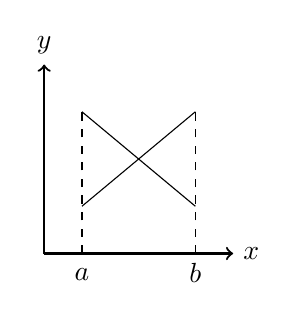
\begin{tikzpicture}[scale=0.6]
            \draw[->,thick] (0,0)--(4,0) node[right]{$x$};
            \draw[->,thick] (0,0)--(0,4) node[above]{$y$};
            \draw[dashed] (0.8,0)--(0.8,3);
            \draw[dashed] (3.2,0)--(3.2,3);

            \draw (0.8,1)--(3.2,3);
            \draw (0.8,3)--(3.2,1);

            \node[below, yshift=-2pt] at (0.8,0) {$a$};
            \node[below] at (3.2,0) {$b$};
            \end{tikzpicture}

            \\[12pt]

            \hspace{40pt} (d) & \hspace{40pt} (e) & \\[6pt]

            %----------------- D -----------------
            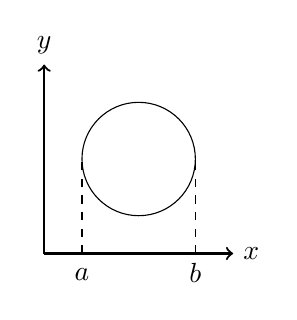
\begin{tikzpicture}[scale=0.6]
            \draw[->,thick] (0,0)--(4,0) node[right]{$x$};
            \draw[->,thick] (0,0)--(0,4) node[above]{$y$};
            \draw[dashed] (0.8,0)--(0.8,2);
            \draw[dashed] (3.2,0)--(3.2,2);

            \draw (2,2) circle (1.2);

            \node[below, yshift=-2pt] at (0.8,0) {$a$};
            \node[below] at (3.2,0) {$b$};
            \end{tikzpicture}

            %----------------- E -----------------
            &
            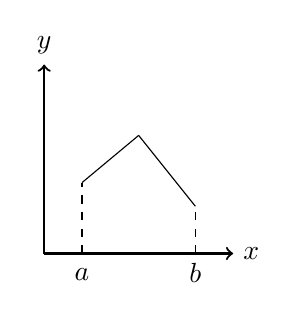
\begin{tikzpicture}[scale=0.6]
            \draw[->,thick] (0,0)--(4,0) node[right]{$x$};
            \draw[->,thick] (0,0)--(0,4) node[above]{$y$};
            \draw[dashed] (0.8,0)--(0.8,1.5);
            \draw[dashed] (3.2,0)--(3.2,1);

            \draw (0.8,1.5)--(2,2.5);
            \draw (2,2.5)--(3.2,1);

            \node[below, yshift=-2pt] at (0.8,0) {$a$};
            \node[below] at (3.2,0) {$b$};
            \end{tikzpicture}
            &
        \end{tabularx}
    \end{center}
}

% Define a resposta correta
\newcommand{\resposta}{A}

% Lógica condicional para exibição
\ifdefstring{\atividade}{lista}{%
    \alternativas
    \vspace{0.5em}
    
    \noindent\textbf{Resposta:} letra \textbf{\resposta}.
}{%
    \ifdefstring{\modo}{objetivo}{%
        \alternativas
    }{%
        % modo = discursiva → não mostra alternativas
    }
}
\end{exercicioBanco}

